\documentclass[12pt]{article} % For LaTeX2e
\usepackage{nips11submit_e,times}
\usepackage{graphicx}
%\documentstyle[nips10submit_09,times,art10]{article} % For LaTeX 2.09

\usepackage{amsmath, amsthm, amssymb}
\usepackage{graphicx}
\usepackage{hyperref}

\newtheorem{prob}{Problem}
\newtheorem*{prop}{Proposition}
\newtheorem*{obs}{Observation}
\newtheorem*{lemma}{Lemma}
\newtheorem*{defn}{Definition}
\newtheorem*{example}{Example}
\newtheorem*{theorem}{Theorem}
\newtheorem*{cor}{Corollary}
\newtheorem*{claim}{Claim}

\newcommand{\brk}[1]{\{#1\}}
\newcommand{\res}{\text{res}}
\newcommand{\dt}{\; \text{d}}
\newcommand{\sq}{\sqrt}
\newcommand{\C}{\mathbb{C}}
\newcommand{\D}{\mathbb{D}}
\newcommand{\R}{\mathbb{R}}
\newcommand{\Q}{\mathbb{Q}}
\newcommand{\N}{\mathbb{N}}
\newcommand{\Z}{\mathbb{Z}}
\newcommand{\sm}{\setminus}
\newcommand{\F}{\mathbb{F}}
\newcommand{\GF}{\text{GF}}
\newcommand{\RS}{\text{RS}}
\newcommand{\lr}[1]{\left (#1 \right )}
\newcommand{\abs}[1]{\left | #1 \right |}
\newcommand{\floor}[1]{\lfloor #1 \rfloor}
\newcommand{\length}{\text{length}}


\title{Machine Learning Toolbox for Feature Extraction and Inference}
\author{Yo Sup ``Joseph'' Moon, Dana Modzelewski, William Chambers, Claudia Friedsam}

\newcommand{\fix}{\marginpar{FIX}}
\newcommand{\new}{\marginpar{NEW}}

\nipsfinalcopy % Uncomment for camera-ready version

\begin{document}
\maketitle


\begin{center}
CS51 Final Project March 25 Draft \\
Due 11:59PM, March 25\textsuperscript{th}, 2012.  
\end{center}


\section{Brief Overview}
 
We want to implement two different methods for unsupervised learning with the goal to extract information from high dimensional data. The algorithms we chose are principal component analysis and k-means clustering.
We want to implement the basic algorithms, test and compare them on a set of diverse data and investigate their performance. We plan to address the limitations we identified by extending the algorithms with straightforward solutions like e.g. heuristics or optimization methods.
In a last step we try to apply our algorithms to address a real world problem like handwriting or object recognition.

\section{Feature}
\begin{enumerate}

	\item K-means 
	
	\emph{Fundamental Features:} 
		\begin{itemize}
			\item K-means algorithm
			\item Test functions
			\item Evaluation methods to examine performance 
		\end{itemize}
	\emph{Possible Extensions:}
		\begin{itemize}
			\item Heuristic or genetic algorithm for optimization
			\item Explore variations of k-means, e.g. density based k-		means, soft k-means 
		\end{itemize}
	\item Principal Component Analysis (PCA)\\
	\emph{Fundamental Features:}
		\begin{itemize}
			\item PCA algorithm
			\item Eigenvector Finding: can we find suitable time-efficient 			algorithm that suits our needs?  
			\item Test functions: sanity check on small-dimensional data. Test robustness of feature extraction: how much of the ``useful'' features of the data preserved?  
		\end{itemize}

	
	 
	\item Common Features: \\
		\emph{Fundamental Features:}
		\begin{itemize}
			\item Method to load and prepare data to be used 
			\item GUI to load data, pick the method, adjust input parameters, visualize results and performance for both methods 
			\item Testing performance of model: k-fold cross validation, logistic regression 
		\end{itemize}
		
		Possible Extensions:
		\begin{itemize}
			\item Extension for handling a variety of different types of data 
			\item GUI elements for real world problems: end goal is to produce a standalone, platform-independent executable program in Windows/UNIX environment  
		\end{itemize}


\end{enumerate}



\section{Draft Technical Specification}

We will be implementing our algorithms in Python, using vim and standard 
UNIX terminal environment to run our code. Our code will be shared and kept up-to-date via a Github repository. 
The modularity of our project arises naturally in the separate implementations of k-means and Principal Component Analysis algorithms. Both algorithms will be a modular component, and can be used for any part of the inference step in application to the data.   

\begin{itemize}
	\item K-means is a clustering method that aims at dividing data sets of n data points into  k clusters which consist of similar points. This is done by assigning each data point to the cluster with the nearest mean.

	\item Another algorithm that we will implement is Principal Component Analysis (PCA).  PCA takes a high dimensional dataset and compresses it by an orthogonal projection of the data and to the principal subspace, a lower dimensional linear space, such that the variance of the projected data is maximized.
The PCA algorithm begins by finding the covariance matrix, S, of the dataset.  We then find the M eigenvectors of S which correspond to the M largest eigenvalues (if the data is of dimensionality $D$, then $M < D$).  The eigenvectors are the principal components onto which we project the data.
\end{itemize}
\begin{center}
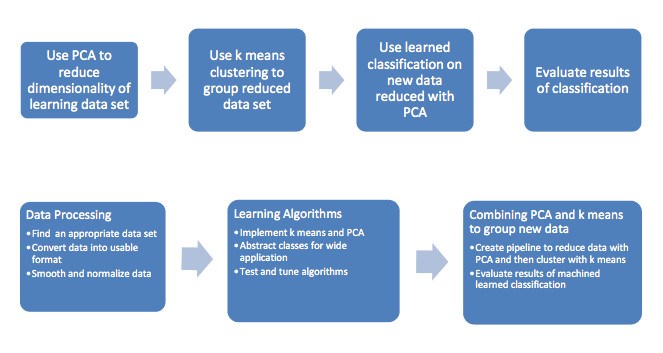
\includegraphics[width=125mm]{flowchart.png}
\end{center}

\subsection{Read Data Module}
\emph{Functions:}
\begin{itemize}
	\item Read file into array 
	\item Perform data clean up (remove outliers, smoothing, etc)
	\item Export Data 
\end{itemize}

\emph{Exceptions:}
\begin{itemize}
	\item Can't read/find file
	\item File contains ill-defined data 
	\item Cleanup failed
	\item Can't write file 
\end{itemize}


\subsection{Description of K-means Module}
Description of K-means algorithm 

\begin{itemize}
	\item Create initial random partition of $n$ data points in $k$ clusters
	\item Calculate centroids $C$ of $k$ clusters
	\item Initialize $C_{old}$ with empty list 
	\item While $C \neq C_{old}$ \textbf{do}:
		\begin{itemize}
			\item $C_{old} \gets C$
			\item Reassign data points to closest cluster centroid 
			\item Calculate $C$ for new clusters 
		\end{itemize}
	\item Return $C$ and $k.$ 
\end{itemize}

\emph{K-means Functions:}
\begin{itemize}
	\item Initialize Clusters
	\item Get centroids of partitioned data 
	\item Calculate distances of points to centroids 
	\item Reassign points to closest clusters 
	\item Export data 
\end{itemize}
\emph{Exceptions:}
\begin{itemize}
	\item Number of clusters too big 
	\item Empty clusters 
	\item Can't write file 
\end{itemize}


\subsection{K-means Evaluation Module}
As a starting point we look at two criteria to investigate how well the clustering works. The first step is to look at the density of the clusters to see how compacted the clusters are. As a second criteria we will determine the silhouette, which is describing how distant the points in a specific cluster are from the other clusters to investigate the separation of the clusters.

\emph{Functions:}
	\begin{itemize}
		\item Calculate Density 
		\item Silhouette
	\end{itemize}


\subsection{Description of PCA Module}
\emph{PCA Functions:}
\begin{itemize}
	\item Calculate covariance matrix, $S$
	\item Find $M$ largest eigenvalues of $S$
	\item Find eigenvectors corresponding to eigenvalues 
	\item Project data onto eigenvectors
	\item Export Data 
\end{itemize}

\emph{Exceptions:}
\begin{itemize}
	\item Can't compute covariance matrix 
	\item Can't find eigenvalues for covariance matrix
	\item Can't write file 
\end{itemize}

\subsection{PCA Evaluation Module}
As a preliminary criterion for determining the success of our PCA algorithm, we will look at the variances from projecting the data onto the principal components.
\emph{Functions}
\begin{itemize}
	\item Calculate variances 
\end{itemize}


\subsection{Test Module}
\emph{Functions:}
	\begin{itemize}
		\item Test functions in k-means module  
		\item Test functions in PCA module 
	\end{itemize}



\section{What is next?}

Since our project will be implemented in Python, we will need to take additional time to familiarize ourselves with the language.  To do this we will use the Python manual as one of our main resources.  In addition, we will also read through examples of well-written machine learning Python code such as that found at \url{http://norvig.com/sudoku.html}.  We plan to use Vim in a standard Unix environment when writing our code and we will be sharing our code with one another using GitHub.

In order to begin working on our project it will be very important for us to identify a dataset.  Without this we will not be able to test our algorithms in any meaningful way nor compare the results of one algorithm with the results of another.  As a preliminary dataset, we would like to use that provided in the second assignment of CS 181, which is perfect for our needs. This is a subset of the MNIST Database, a large dataset of handwritten numbers (available at \url{http://yann.lecun.com/exdb/mnist/}).  This dataset is ideal as it contains training, validation, and test sets which will allow us begin working with the data right away.  As we get further along with our project we will want to expand our dataset as we see fit.


\end{document}